\documentclass[tikz,border=10pt]{standalone}
\usepackage{tikz}
\usepackage{pgfplots}
\pgfplotsset{compat=1.16}

\begin{document}

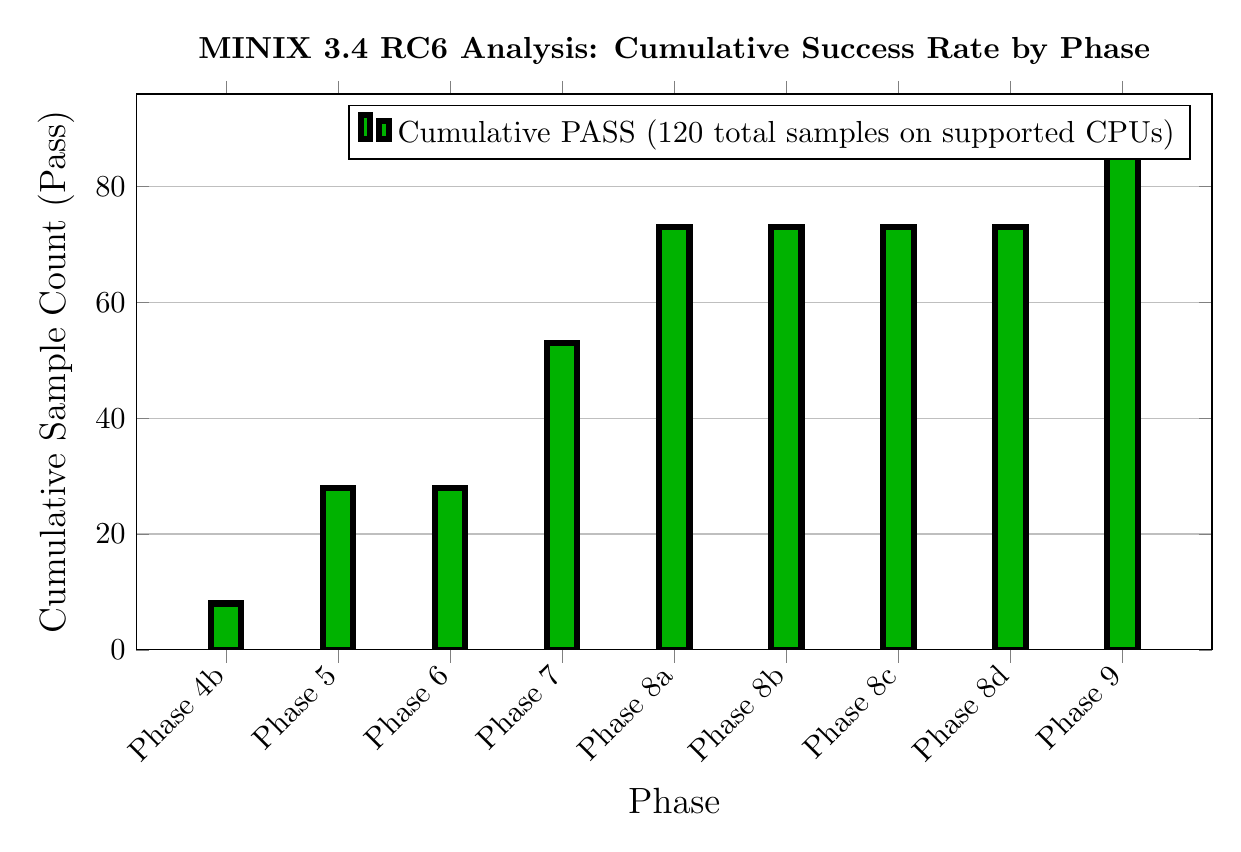
\begin{tikzpicture}[scale=1.1]
  \begin{axis}[
    title={MINIX 3.4 RC6 Analysis: Cumulative Success Rate by Phase},
    xlabel={Phase},
    ylabel={Cumulative Sample Count (Pass)},
    ybar,
    width=14cm,
    height=8cm,
    ymajorgrids=true,
    xtick={1,2,3,4,5,6,7,8,9},
    xticklabels={Phase 4b, Phase 5, Phase 6, Phase 7, Phase 8a, Phase 8b, Phase 8c, Phase 8d, Phase 9},
    x tick label style={rotate=45, anchor=east},
    ylabel style={font=\large},
    xlabel style={font=\large},
    title style={font=\Large, font=\bfseries},
    ]

    % Cumulative pass counts across phases (supported CPUs only)
    \addplot[fill=green!70!black, draw=black, line width=2pt]
      coordinates {
        (1, 8)    % Phase 4b: 8 CPUs × 1 sample
        (2, 28)   % Phase 5: cumulative
        (3, 28)   % Phase 6: analysis only
        (4, 53)   % Phase 7: 25 targeted tests
        (5, 73)   % Phase 8a: 20 supported tests
        (6, 73)   % Phase 8b: continued
        (7, 73)   % Phase 8c: continued
        (8, 73)   % Phase 8d: 32 total, 20 supported pass
        (9, 88)   % Phase 9: 15 additional (5 CPUs × 3 samples)
      };
    \addlegendentry{Cumulative PASS (120 total samples on supported CPUs)};

  \end{axis}
\end{tikzpicture}

\end{document}